\documentclass{beamer}

\usepackage[utf8]{inputenc}
%\usepackage{beamerthemesplit}
\usepackage{url}
\usepackage{tikz}
\usepackage{alltt}
\usepackage{listings}
\usepackage{marvosym}
\usepackage{color}
\usepackage[multidot]{grffile}
\usepackage{multirow}
\usepackage{array}
\usepackage{setspace}
\usepackage{hyperref}
\usepackage{verbatim}
\usepackage{fancyvrb}
%\hypersetup{colorlinks=true, linkcolor=blue,  anchorcolor=blue,  
%citecolor=blue, filecolor=blue, menucolor=blue, pagecolor=blue,  
%urlcolor=blue} 
\lstset{keywordstyle=\bfseries\color{brown},
        stringstyle=\ttfamily,
        commentstyle=\color{blue}\textit,
        showstringspaces=false}

\useoutertheme{}
\usetheme{Madrid}
\graphicspath{{pics/}{global/}
{pics/I/}{pics/A1/}{pics/A2/}{pics/A3/}{pics/A4/}{pics/A5/}{pics/A6/}{pics/A7/}
}

\logo{
\includegraphics[height=1cm]{ProcessHorizontal}} 

\institute{Center for Computation and Technology\\Louisiana State University, Baton Rouge, LA}

\setbeamertemplate{navigation symbols}{} 

\title{CSC 7700: Scientific Computing}

% We want to use the infolines outer theme because it does not use a lot of
% space, but it also tries to print an institution and the slide
% numbers (which we might not want to show). Therefore, we here redefine the
% footline ourselfes - mostly a copy & paste from
% /usr/share/texmf/tex/latex/beamer/themes/outer/beamerouterthemeinfolines.sty
\defbeamertemplate*{footline}{infolines theme without institution and slide numbers}
{
  \leavevmode%
  \hbox{%
  \begin{beamercolorbox}[wd=.25\paperwidth,ht=2.25ex,dp=1ex,center]{author in head/foot}%
    \usebeamerfont{author in head/foot}\insertshortauthor
  \end{beamercolorbox}%
  \begin{beamercolorbox}[wd=.5\paperwidth,ht=2.25ex,dp=1ex,center]{title in head/foot}%
    \usebeamerfont{title in head/foot}\insertshorttitle
  \end{beamercolorbox}%
  \begin{beamercolorbox}[wd=.25\paperwidth,ht=2.25ex,dp=1ex,center]{date in head/foot}%
    \usebeamerfont{date in head/foot}\insertshortdate{}
  \end{beamercolorbox}}%
  \vskip0pt%
}

% Some useful commands
\newcommand{\abspic}[4]
 {\vspace{ #2\paperheight}\hspace{ #3\paperwidth}\includegraphics[height=#4\paperheight]{#1}\\
  \vspace{-#2\paperheight}\vspace{-#4\paperheight}\vspace{-0.0038\paperheight}}

\newcommand{\picw}[4]{{
 \usebackgroundtemplate{
 \color{black}\vrule width\paperwidth height\paperheight\hspace{-\paperwidth}\hspace{-0.01\paperwidth}
 \hspace{#4\paperwidth}\includegraphics[width=#3\paperwidth, height=\paperheight]{#1}}\logo{}
 \frame[plain]{\frametitle{#2}}
}}
\newcommand{\pic}[2]{\picw{#1}{#2}{}{0}}

\newcommand{\question}[1]{\frame{\frametitle{#1}
 \begin{centering}\Huge #1\\\end{centering}
}}



%\usecolortheme[RGB={200,200,200}]{structure}

\subtitle[Module D]{{\large Module D: Simulations and Application Frameworks}\\*[0.3em]Lecture 2: Simulating Complex Systems}
\author[Peter Diener]{Dr Peter Diener}
\date{November 15, 2013}
\usecolortheme[RGB={45,160,140}]{structure}

\begin{document}

\frame{\titlepage}

\section*{Outline}
\frame{\tableofcontents}

\section{Goals}
\frame{\frametitle{}\begin{centering}\LARGE\insertsectionhead\\\end{centering}}

\frame[containsverbatim]{ \frametitle{Goals}
  \begin{itemize}
    \item Lecture 1 described the application scientist's point of view.
    \item This lecture discusses the \emph{computer science issues} in
          simulations and simulation codes.
      \begin{itemize}
        \item Parallel computing (algorithm design)
        \item Component model (software design)
      \end{itemize}
    \item In most research groups, a computer scientist is an expensive
          luxury; only large projects can afford computer scientists.
  \end{itemize}
}

\section{Summary}
\frame{\frametitle{}\begin{centering}\LARGE\insertsectionhead\\\end{centering}}

\frame[containsverbatim]{ \frametitle{Summary}
  \begin{itemize}
    \item To go from physics to a simulation, one usually
      \begin{enumerate}
        \item Finds a mathematical model (e.g.\ PDEs) expressing the physics.
        \item Discretise the model (e.g.\ PDEs).
        \item Implement the discretised equations on a supercomputer
      \end{enumerate}
    \item Many simulation codes have a similar structure.
    \item Many supercomputers have a similar architecture.
  \end{itemize}
}

\section{Parallel Computing}
\frame{\frametitle{}\begin{centering}\LARGE\insertsectionhead\\\end{centering}}

\frame[containsverbatim]{ \frametitle{HPC History}
  \begin{minipage}[b]{7.5cm}
    \begin{itemize}
      \item Before MPI: \emph{Vector architectures}, e.g.\ Cray Y-MP (until
            $\sim 1992$).
      \item In the Y-MP, the vector length was 64 words (1 word is 64 bits)
            and it had 8 vector registers.
      \item Much more efficient than scalar processors (compare conveyor belt
            vs.\ hand assembly).
      \item Disadvantages: too inflexible for dynamic data structures, too
            expensive due to custom designed (low volume) hardware and memory
            system.
    \end{itemize}
  \end{minipage}
  \raisebox{8.5em}{
    \begin{minipage}[t]{4.0cm}
      \includegraphics[width=3.8cm]{pics/cray-ymp}\vspace{0.5em}\\
      \includegraphics[width=3.8cm]{pics/assembly-line}\\
    \end{minipage}
  }
}

\frame[containsverbatim]{ \frametitle{HPC History}
  \begin{itemize}
    \item After vector machines \emph{cluster architectures} became prevalent
         (e.g.\ Cray T3D, 1993 and CM-5, 1991).
    \item Basic idea: have many simple nodes connected by high-speed network.
    \item Nodes need to communicate (\emph{exchange messages}) during
          computation.
    \item Also called \emph{Beowulf architecture}, especially if only
          cheap commodity components are used.
    \item The need for communication lead to the development of MPI.
  \end{itemize}
}

\frame[containsverbatim]{ \frametitle{MPI: Message Passing Interface}
  \includegraphics[width=1.5cm]{pics/mpilogogreen}\hfill
  \includegraphics[width=2cm]{pics/mpi2-logo}
  \begin{itemize}
    \item MPI is an Application Programming Interface (API); It is
          \underline{\bf{THE}} industry standard for parallel HPC programming.
    \item Supported on all important HPC platforms.
    \item Very successful (standard since 1994) since it makes it 
          \emph{possible} to implement efficient parallel algorithms.
    \item Note the emphasis on \emph{possible} rather than \emph{easy}.
    \item \begin{verbatim}www.mpi-forum.org\end{verbatim}
  \end{itemize}
}

%\frame[containsverbatim]{ \frametitle{MPI Programming}
%  \begin{itemize}
%    \item Each process runs an independent copy of the program.
%    \item Each copy has a unique number assigned to it ($0\ldots N-1$).
%    \item The program has to divide the total workload into $N$ pieces and
%          assign one to each process.
%    \item The processes can talk to each other \emph{only} by exchanging
%          messages.
%    \item MPI hides low-level system dependent communication details from the
%          programmer.
%    \item MPI messages are (by default) \emph{ordered} and \emph{reliable}.
%  \end{itemize}
%}
%
%\frame[containsverbatim]{ \frametitle{MPI Programming}
%  \begin{itemize}
%    \item Message Passing is very common, even in the real world:
%      \begin{itemize}
%         \item Letters via the post office.
%         \item E-mail.
%         \item Phone voice mail messages.
%         \item Newspapers.
%      \end{itemize}
%    \item However, these are NOT message passing -- instead they are 
%          \emph{streams} or \emph{interactive}:
%      \begin{itemize}
%        \item Phone conversation.
%        \item Watching TV.
%        \item Google Docs.
%        \item WoW.
%      \end{itemize}
%  \end{itemize}
%}
%
%\frame[containsverbatim]{ \frametitle{MPI Programming}
%  \begin{itemize}
%    \item Example: Distributing an array over multiple MPI processes.
%    \item Assuming: 50 elements and 5 processes; A possible way would
%          be for each process to \emph{own} 10 elements.
%    \item We can perform two operations on arrays: set-element and get-element.
%          When a process wants to set or get an element owned by another
%          process we have to implement these operations with MPI.
%    \item set-element(n,x):
%      \begin{enumerate}
%        \item Determine which process owns element n.
%        \item Send message to that process containing index n and value x.
%        \item Check whether message has been received.
%        \item If so, set element n to x on the process that owns the element.
%      \end{enumerate}
%  \end{itemize}
%}
%
%\frame[containsverbatim]{ \frametitle{MPI Programming}
%  \begin{itemize}
%    \item x = get-element(n):
%      \begin{enumerate}
%        \item Determine which process owns element n.
%        \item Send message to that process requesting element n.
%        \item Check whether message has been received.
%        \item If so, the process that owns element n will get it...
%        \item ...and send a message back with value x.
%        \item Wait for the result.
%      \end{enumerate}
%    \item In reality it's very inefficient to send messages with individual
%          elements. It's better to send \emph{batches} of elements to reduce
%          \emph{latency}.
%    \item Without going into details this shows that MPI programming is
%          complicated.
%    \item With a large investment of effort it can be made very efficient.
%    \item Most alternatives to MPI are less efficient, especially on 
%          1,000+ or 10,000+ processes.
%    \item \begin{minipage}[t]{8cm}
%            Alternatives are e.g.\ Co-Array Fortran (CAF) or Unified Parallel
%            C (UPC).
%          \end{minipage}
%  \end{itemize}
%}

\frame[containsverbatim]{ \frametitle{Amdahl's Law}
  \begin{minipage}[b]{6cm}
    \begin{itemize}
      \item $P$: Fraction of code that can be parallelised.
      \item $N$: Number of processors used.
      \item Amdahl's law:
    \end{itemize}
    \[
      S = \frac{1}{(1-P)+P/N}
    \]
  \end{minipage}
  \raisebox{-1.5em}{
    \begin{minipage}[t]{5cm}
      \includegraphics[width=4.8cm]{amdahls-law}
    \end{minipage}
  }
  \begin{itemize}
    \item When running on $N$ processes, not necessarily $N$ times as 
          fast.
    \item Overhead and non-parallelisable part of the code determines maximum
          possible parallel speedup.
    \item 100,000-fold speedup requires $>99.999$\% parallelisation.
  \end{itemize}
}

\frame[containsverbatim]{ \frametitle{MPI Programming}
  \begin{itemize}
    \item Efficient MPI parallelisation is complex and tedious.
    \item Requires re-designing data type layouts and APIs (and then
          rewriting the program).
    \item To ensure correctness, need good encapsulation of parallelism
          and understanding of advanced programming concepts.
    \item Design and implementation needs to be carefully thought out
	  in order to ensure extensibility and portability.
  \end{itemize}
}

\frame[containsverbatim]{ \frametitle{Domain Decomposition}
  \begin{minipage}[b]{6.5cm}
    \begin{itemize}
      \item In a domain decomposition scheme, the discrete elements (points,
            cells, particles, \ldots) are distributed among the processors.
      \item Each process handles only those that it \emph{owns} (without
            requiring communication).
      \item Accessing elements from neighboring processes requires
            communication (e.g.\ at domain boundaries).
    \end{itemize}
  \end{minipage}
  \raisebox{2.0em}{
    \begin{minipage}[t]{4.5cm}
      \includegraphics[width=4.3cm]{wire-frame}
    \end{minipage}
  }
}

\frame { \frametitle{Domain Decomposition}
 Without Ghostzones:\\
 \begin{centering}\includegraphics[width=9cm]{1dnoghost}\\\end{centering}
 With Ghostzones:\\
 \begin{centering}\includegraphics[width=9cm]{withghost}\\\end{centering}
}

\frame { \frametitle{Domain decomposition}
 \begin{centering}\includegraphics[width=11cm]{domain_decomposition}\\\end{centering}
}

\frame[containsverbatim]{ \frametitle{The Wave Equation}
  Approximating the pressure $P(x,t)$ with a grid function $P_i^{(n)}$.
  \begin{minipage}[b]{3.05cm}
    \includegraphics[width=3cm]{pics/discretisation}
  \end{minipage}
  \raisebox{8em}{
  \begin{minipage}[t]{8.5cm}
    \begin{eqnarray}
      \frac{\partial^2 P}{\partial t^2} & = & 
       v^2\frac{\partial^2 P}{\partial x^2} \nonumber \\
      & \Downarrow & \nonumber \\
      \frac{P_i^{(n+1)}-2 P_i^{(n)}+P_i^{(n-1)}}{\Delta t^2} & = &
      v^2\frac{P_{i+1}^{(n)}-2 P_i^{(n)}+P_{i-1}^{(n)}}{\Delta x^2} \nonumber
    \end{eqnarray}
  \end{minipage}}
  The error from this time and space discretisation is $O(h^2)$.
}

\frame{ \frametitle{Wave Equation: Algorithm Illustration}
 \begin{columns}[t]
 \column{.7\textwidth}
   \begin{figure}[!htp]
   \begin{center}
     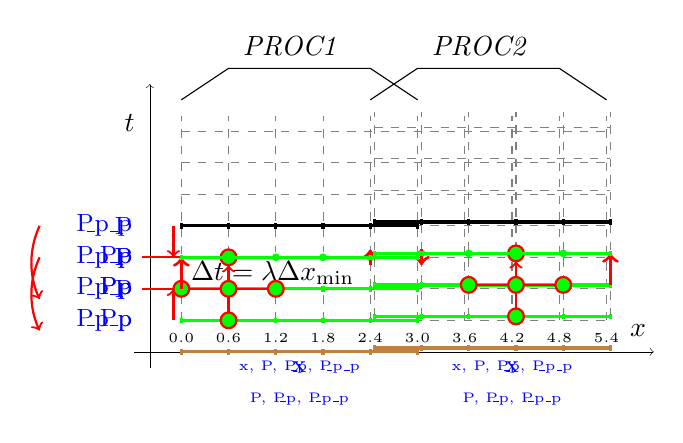
\begin{tikzpicture}

       %\draw[->] (0,0) -- (1,1);
       % Step 1: axes and grid
       \draw[->,very thin] (-.6,-.4) -- (6,-.4);
       \draw[->,very thin] (-.4,-.6) -- (-.4,3);
       \draw[left=2pt] (-.4,2.5)   node {$t$};
       \draw[above=2pt] (5.8,-0.4) node {$x$};

       \uncover<1>{
         \draw[xstep=.6cm,ystep=.4cm,gray,dashed]
              (0,0) grid(5.4cm,2.6cm);
       }%

       % Step 2: splitting between two processors
       \uncover<2->{
         \draw (0,2.8) -- (.6,3.2) -- (2.4,3.2) -- (3,2.8);
         \draw[above=1pt] (1.4,3.2) node {\emph{PROC1}};

         \draw[xshift=2.4cm] (0,2.8) -- (.6,3.2) -- (2.4,3.2) -- (3,2.8);
         \draw[above=1pt] (3.8,3.2) node {\emph{PROC2}};
       }%
       \uncover<2-4>{
         \draw[xstep=.6cm,ystep=.4cm,gray,dashed]
              (0,0)   grid (3.0cm,2.6cm);
         \draw[xstep=.6cm,ystep=.4cm,gray,dashed,xshift=0.05cm,yshift=0.05cm]
              (2.4,0) grid (5.4cm,2.6cm);
       }%

       % Step 3: memory "allocations" 
       \uncover<3>{
         \draw[color=blue] (1.5,-0.6) node {\tiny x, P, P\!\!\_p, P\!\!\_p\_p};
         \draw[color=blue] (4.2,-0.6) node {\tiny x, P, P\!\!\_p, P\!\!\_p\_p};
       }%

       % Step 4: CoordBase / CartGrid3D
       \uncover<4->{
          \foreach \x in {0.0,0.6,1.2,1.8,2.4,3.0,3.6,4.2,4.8,5.4}
            \draw (\x cm,-0.4cm) node[anchor=south] {{\tiny $\x$}};
          \draw[very thick,color=brown,xstep=0.6cm,ystep=1cm,yshift=-0.4cm]
            (0cm,-1pt) grid (3.0cm,1pt);
          \draw[color=blue] (1.5,-0.6) node {\small x};

          \draw[very thick,color=brown,xstep=0.6cm,ystep=1cm,xshift=2.45cm,yshift=-0.35cm]
            (0cm,-1pt) grid (3.0cm,1pt);
          \draw[color=blue] (4.2,-0.6) node {\small x};
       }
       \uncover<4-5>{
         \draw[color=blue] (1.5,-1.0) node {\tiny P, P\!\!\_p, P\!\!\_p\_p};
         \draw[color=blue] (4.2,-1.0) node {\tiny P, P\!\!\_p, P\!\!\_p\_p};
       }%

       % Step 5: Time
       \uncover<5->{
         \draw[xstep=.6cm,ystep=.4cm,gray,dashed]
              (0,0)   grid (3.0cm,2.6cm);
         \draw[xstep=.6cm,ystep=.4cm,gray,dashed,xshift=0.05cm,yshift=0.05cm]
              (2.4,0) grid (5.4cm,2.6cm);
       }%
       \uncover<5>{
         \scope[color=red,thick,fill=white]
           \draw (-0.5,0.4) -- (0.0,0.4);
           \draw (-0.5,0.8) -- (0.0,0.8);
           \draw[->] (-0.1,1.2) -- (-0.1,0.8);
           \draw[<-] (-0.1,0.4) -- (-0.1,0.0);
         \endscope
         \draw (0,0.6) node[anchor=west,fill=white] {$\Delta t = \lambda\Delta x_{\min}$};
       }

       % Step 6: Initial data routines
       \uncover<6->{
         \scope[very thick,color=green,xstep=0.6cm,ystep=1cm]
          \draw[xshift=0cm,yshift=0cm]       (0cm,-1pt) grid (3.0cm,1pt);
          \draw[xshift=2.45cm,yshift=0.05cm] (0cm,-1pt) grid (3.0cm,1pt);        
          \draw[xshift=0cm,yshift=0.4cm]     (0cm,-1pt) grid (3.0cm,1pt);
          \draw[xshift=2.45cm,yshift=0.45cm] (0cm,-1pt) grid (3.0cm,1pt);        
          \draw[xshift=0cm,yshift=0.8cm,color=black]     (0cm,-1pt) grid (3.0cm,1pt);
          \draw[xshift=2.45cm,yshift=0.85cm,color=black] (0cm,-1pt) grid (3.0cm,1pt);
         \endscope
       }%
       \uncover<6>{
         \scope[color=blue]
           \draw (-0.5,0.0) node[anchor=east] {\small P\!\!\_p};
           \draw (-0.5,0.4) node[anchor=east] {\small P};
           \draw (-0.5,0.8) node[anchor=east] {\small P\!\!\_p\_p};
         \endscope
       }

       % Step 7: Layers rotation
       \uncover<7>{
         %\draw[thick,color=red,->] (-0.5,-0.1) arc (-25:25:1.1cm);
         \draw[thick,color=red,->] (-1.8, 0.8) arc (155:205:1.1cm);
       }
       \uncover<7-11>{
         \scope[color=blue]
           \draw (-0.5,0.0) node[anchor=east] {\small P\!\!\_p\_p};
           \draw (-0.5,0.4) node[anchor=east] {\small P\!\!\_p};
           \draw (-0.5,0.8) node[anchor=east] {\small P};
         \endscope
       }

       % Step 8: Evaluation of RHS
       \uncover<8>{
         \scope[draw=red,thick,fill=green]
           \fill (1.2,0.8) circle (0.05cm);
           \fill (1.8,0.8) circle (0.05cm);
           \fill (2.4,0.8) circle (0.05cm);
           \draw (0.0,0.4) -- (1.2,0.4);
           \draw[->] (0.6,0.0) -- (0.6,0.7);
           \filldraw (0.6,0.8) circle (0.1cm);
           \filldraw (0.6,0.0) circle (0.1cm);
           \filldraw (0.0,0.4) circle (0.1cm);
           \filldraw (0.6,0.4) circle (0.1cm);
           \filldraw (1.2,0.4) circle (0.1cm);

           % second processor:
           \scope[xshift=0.05cm,yshift=0.05cm]
             \fill (3.0,0.8) circle (0.05cm);
             \fill (3.6,0.8) circle (0.05cm);
             \fill (4.8,0.8) circle (0.05cm);
             \scope[xshift=3.6cm]
               \draw (0.0,0.4) -- (1.2,0.4);
               \draw[->] (0.6,0.0) -- (0.6,0.7);
               \filldraw (0.6,0.8) circle (0.1cm);
               \filldraw (0.6,0.0) circle (0.1cm);
               \filldraw (0.0,0.4) circle (0.1cm);
               \filldraw (0.6,0.4) circle (0.1cm);
               \filldraw (1.2,0.4) circle (0.1cm);
             \endscope
           \endscope
         \endscope
       }%

       % Step 9: Ghost zones
       \uncover<9>{
         \scope[very thick,color=green,xstep=0.6cm,ystep=1cm]
          \draw[xshift=0.6cm,yshift=0.8cm]       (0cm,-1pt) grid (1.8cm,1pt);
          \draw[xshift=3.05cm,yshift=0.85cm] (0cm,-1pt) grid (1.8cm,1pt);        
          \draw[->,color=red] (2.4,0.7) -- (2.4,0.9);
          \draw[->,color=red] (3.05,0.9) -- (3.05,0.7);
         \endscope
       }%

       % Step 10: Boundary conditions
       \uncover<10>{
         \scope[very thick,color=green,xstep=0.6cm,ystep=1cm]
          \draw[xshift=0.6cm,yshift=0.8cm]       (0cm,-1pt) grid (2.4cm,1pt);
          \draw[xshift=2.45cm,yshift=0.85cm] (0cm,-1pt) grid (2.4cm,1pt);        
          \draw[->,color=red] (0.0,0.4) -- (0.0,0.8);
          \draw[->,color=red] (5.45,0.45) -- (5.45,0.85);
         \endscope
       }%

       % Step 11: Output data
       \uncover<11->{
         \scope[very thick,color=green,xstep=0.6cm,ystep=1cm]
          \draw[xshift=0cm,yshift=0.8cm]     (0cm,-1pt) grid (3.0cm,1pt);
          \draw[xshift=2.45cm,yshift=0.85cm] (0cm,-1pt) grid (3.0cm,1pt);        
         \endscope
       }

       % Step 12: Advance to the next time level
       \uncover<12->{
         \scope[very thick,color=green,xstep=0.6cm,ystep=1cm]
          \draw[xshift=0cm,yshift=1.2cm,color=black]     (0cm,-1pt) grid (3.0cm,1pt);
          \draw[xshift=2.45cm,yshift=1.25cm,color=black] (0cm,-1pt) grid (3.0cm,1pt);
          \draw[xshift=0cm,yshift=0.8cm]     (0cm,-1pt) grid (3.0cm,1pt);
          \draw[xshift=2.45cm,yshift=0.85cm] (0cm,-1pt) grid (3.0cm,1pt);        
         \endscope
       }
       \uncover<12>{
         \scope[color=blue]
           \draw (-0.5,0.4) node[anchor=east] {\small P\!\!\_p};
           \draw (-0.5,0.8) node[anchor=east] {\small P};
           \draw (-0.5,1.2) node[anchor=east] {\small P\!\!\_p\_p};
         \endscope
       }

       % Step 13: Layers rotation again
       \uncover<13>{
         %\draw[thick,color=red,->] (-0.5,-0.1) arc (-25:25:1.1cm);
         \draw[thick,color=red,->] (-1.8, 1.2) arc (155:205:1.1cm);
       }
       \uncover<13-13>{
         \scope[color=blue]
           \draw (-0.5,0.4) node[anchor=east] {\small P\!\!\_p\_p};
           \draw (-0.5,0.8) node[anchor=east] {\small P\!\!\_p};
           \draw (-0.5,1.2) node[anchor=east] {\small P};
         \endscope
       }
     \end{tikzpicture}
   \end{center}
   \end{figure}

 \column{.3\textwidth}
   \begin{figure}[!htp]
   \begin{center}
   \vspace{-1cm}
   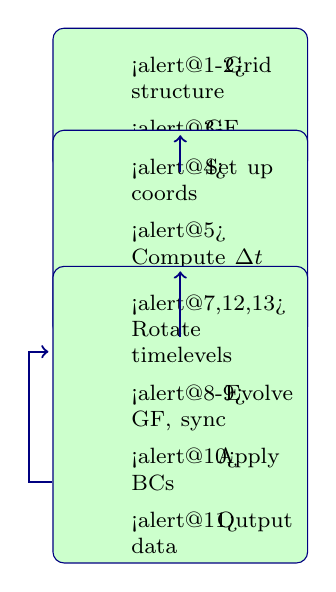
\begin{tikzpicture}
      \draw (0,7) node
      [anchor=north,right,text width=3cm,rounded corners,fill=green!20,draw=blue!50!black] %,inner sep=1ex]
      (begin)
      {\begin{footnotesize}
       \begin{itemize}
       \item[]<alert@1-2> \hspace{-0.5cm} Grid structure
       \item[]<alert@3>   \hspace{-0.5cm} GF allocation
       \end{itemize}
       \end{footnotesize}};

      \draw (0,5.3) node
      [anchor=north,right,text width=3cm,rounded corners,fill=green!20,draw=blue!50!black] %,inner sep=1ex]
      (init)
      {\begin{footnotesize}
       \begin{itemize}
       \item[]<alert@4> \hspace{-0.5cm} Set up coords
       \item[]<alert@5> \hspace{-0.5cm} Compute $\Delta t$
       \item[]<alert@6> \hspace{-0.5cm} Initial data
       \end{itemize}
       \end{footnotesize} };

      \draw[->,thick,draw=blue!50!black] (0,2.15) -- (-0.3,2.15) -- (-0.3,3.8) -- (-0.05,3.8);

      \draw (0,3) node
      [anchor=north,right,text width=3cm,rounded corners,fill=green!20,draw=blue!50!black] %,inner sep=1ex]
      (evol)
      {\begin{footnotesize}
       \begin{itemize}
       \item[]<alert@7,12,13>   \hspace{-0.5cm} Rotate timelevels
       \item[]<alert@8-9>    \hspace{-0.5cm} Evolve GF, sync
       \item[]<alert@10> \hspace{-0.5cm} Apply BCs
       \item[]<alert@11> \hspace{-0.5cm} Output data
       \end{itemize}
       \end{footnotesize} };

      \scope[color=blue!50!black,thick]
        \draw[->,shorten >=2pt] (begin.south) -- (init.north);
        \draw[->,shorten >=2pt] (init.south)  -- (evol.north);
      \endscope
   \end{tikzpicture}
   \end{center}
   \end{figure}
 \end{columns}
}

\frame[containsverbatim]{ \frametitle{Load Balancing}
  \begin{itemize}
    \item In the previous example all processes have to perform the same
          operation at the same time, i.e.\ they progress in \emph{lock step}.
      \begin{itemize}
        \item If one process finish early, it has to idle (wastes time).
        \item If one process finish late, all others have to idle (much worse!)
      \end{itemize}
    \item Remedies: try to distribute load evenly (hard to do if different
          amount of work has to be done for different elements) or
          distribute load dynamically (results in overhead). 
    \item Typical resource allocation problem, very computer sciency,
          requires complex (parallel) data structures.
  \end{itemize}
}

\frame[containsverbatim]{ \frametitle{Ghost Zone Overhead}
  \begin{itemize}
    \item Ghost zones require a memory overhead, since the same array element
          is stored on multiple processes.
    \item In the wave equation example the overhead was 20\%.
    \item In a realistic example (e.g.\ binary black hole evolution) the
          overhead can be much larger:
      \begin{itemize}
        \item Assume $30^3 = 27,000$ grid points per process (3D).
        \item With 5 ghost zones (high order finite differencing) we then 
              have $(30+2\cdot 5)^3 = 40^3 = 64,000$ grid points with ghosts.
       \item Thus we have $40^3-30^3=37,000$ ghost points per process.
       \item This is an overhead of 137\%!
      \end{itemize}
  \end{itemize}
}

\frame[containsverbatim]{ \frametitle{Ghost Zone Overhead}
  \begin{itemize}
    \item We need efficient parallel algorithms for current supercomputers in
          every corner of the program (Amdahl)!
    \item MPI is the first choice for implementing parallel algorithms.
    \item Domain decomposition (e.g.\ with ghost zones) distributes simulation
          data over nodes.
    \item Some important computer science aspects:
      \begin{itemize}
        \item Designing and implementing efficient distributed data types.
        \item Load balancing and scheduling to ensure processors don't idle.
        \item Potentially overlap communication with computation in order to
              hide the latency and overhead of the communication.
      \end{itemize}
  \end{itemize}
}

\section{Component Model}
\frame{\frametitle{}\begin{centering}\LARGE\insertsectionhead\\\end{centering}}

\frame[containsverbatim]{ \frametitle{Simulation Code Requirements}
  \begin{itemize}
    \item Reliability: So that we can trust the results.
    \item Extensibility: So that researchers can add and experiment with new
          ideas.
    \item Usability: So that graduate (or under graduate) students don't waste
          too much time.
    \item Performance: So that we don't waste valuable resources.
  \end{itemize}
}

\frame[containsverbatim]{ \frametitle{Complex simulations}
  \begin{minipage}[b]{7cm}
    \begin{itemize}
      \item Real world problems are complex, not just a single physics system.
      \item Consequently modern simulations may contain several physical models
            at the same time.
      \item Each may have its own set of PDEs and its own discretisation.
      \item How to handle this complexity?
    \end{itemize}
  \end{minipage}
  \begin{minipage}[t]{4.9cm}
    \includegraphics[width=4.7cm]{hurricane}
  \end{minipage}
}

\frame[containsverbatim]{ \frametitle{Example: Long Gamma-Ray Burst}
  \begin{minipage}[t]{4.9cm}
    \vspace{0pt}
    \includegraphics[width=4.7cm]{GRB}
  \end{minipage}
  \begin{minipage}[t]{7.0cm}
    \vspace{0pt}
    \begin{itemize}
      \item General Relativity (black hole).
      \item Relativistic hydrodynamics (star).
      \item Microphyscis, equation of state (shock wave).
      \item Neutrino radiation (cooling, heating).
      \item Magnetic fields (jet formation -- mechanism not yet understood).
      \item Photon radiation (afterglow).
    \end{itemize}
  \end{minipage}
}

\frame[containsverbatim]{ \frametitle{Typical Research Scenario}
  \begin{itemize}
    \item Different models are contributed by different people (each expert
          in his/her area) and then combined into a single code.
    \item Physicists contribute models.
    \item Mathematicians contribute discretisations methods.
    \item Computer scientists need to contribute:
      \begin{itemize}
        \item A software architecture that makes this possible in a safe
              yet efficient manner.
      \end{itemize}
    \item The physicist, mathematician and computer scientist need to work
          closely together (overcome language barrier) in order to achieve a
          good implementation.
  \end{itemize}
}

\frame[containsverbatim]{ \frametitle{Collaboration Problems}
  \begin{itemize}
    \item Example: The Einstein Toolkit (not untypical)
      \begin{itemize}
        \item Parts of the code is 13+ years old.
        \item Graduate students leave after 3 productive years.
        \item Post docs may only be around for 1 or 2 years before moving on.
        \item Many original authors are not available anymore.
        \item Developers distributed over many locations on several continents.
        \item Most physicists/mathematicians are not good programmers.
      \end{itemize}
  \end{itemize}
}

\frame[containsverbatim]{ \frametitle{Component Architecture}
  \begin{itemize}
    \item Split program into independent \emph{components}.
    \item A \emph{framework} provides lean glue between these.
    \item Each component is developed independently by a small group of
          developers.
    \item The end user assembles the components needed to perform the
          simulations.
    \item There is no central control.
    \item There is no authoritative version.
  \end{itemize}
}

\frame[containsverbatim]{ \frametitle{Component Framework}
  \begin{itemize}
    \item Basic principle: \emph{control inversion} where main program
          is provided by framework and components look like libraries.
      \begin{itemize}
        \item No component is ``more important''.
      \end{itemize}
    \item The Framework itself does no real work. It just glues components
          together.
      \begin{itemize}
        \item Components don't interact directly with each other. Only via
              the framework and the rules set by the framework.
      \end{itemize}
  \end{itemize}
}

\frame[containsverbatim]{ \frametitle{Example: The Einstein Toolkit}
  \begin{center}
    \includegraphics[width=5cm]{einsteintoolkit-2}
  \end{center}
  \begin{minipage}[t]{3cm}
    \vspace{0pt}
    \reflectbox{\includegraphics[width=2.8cm]{einsteintoolkit-1}}
  \end{minipage}
  \begin{minipage}[t]{8cm}
    \vspace{0pt}
    \begin{itemize}
      \item Goal: Have state-of-the-art set of tools for Numerical Relativity
                  available as open source.
      \item Organized by the Einstein Consortium.
      \item Open to everyone.
      \item See \underline{\tt{http://einsteintoolkit.org}}
    \end{itemize}
  \end{minipage}
}

\frame[containsverbatim]{ \frametitle{Example: The Einstein Toolkit}
  \begin{center}
    \includegraphics[width=6.2cm]{ETCode}
  \end{center}
}

\frame[containsverbatim]{ \frametitle{The Einstein Toolkit: People}
  \begin{itemize}
    \item About 50 contributors over the past decade, both from physics and
          computer science. Many has left the field.
    \item Currently 95 members from 50 different groups and institutions in
          15 different countries.
    \item Currently 9 maintainers from 6 different sites.
    \item $>250$ publications, $>40 theses$ in physics, astronomy and computer
          science building on these components.
    \item Countless talks at the major astrophysics conferences/meetings are
	  based on these components.
  \end{itemize}
}

\frame[containsverbatim]{ \frametitle{The Einstein Toolkit: Components sampler}
  \begin{itemize}
    \item Evolution systems (both spacetime and matter).
    \item Boundary conditions (both symmetry and physical).
    \item Initial conditions (both spacetime and matter).
    \item Excision/Turduckening.
    \item Wave extraction.
    \item Horizon finding.
    \item Time stepping methods (multiple).
    \item Finite differencing.
    \item Adaptive Mesh Refinement (AMR) driver.
    \item I/O methods (output and checkpoint/restart).
    \item Web server.
    \item Twitter client.
  \end{itemize}
}

\frame[containsverbatim]{ \frametitle{Component Model Summary}
  \begin{itemize}
    \item Modern simulation codes are complex and can contain multiple
          physics models.
    \item The component model can provide the necessary abstraction and
          encapsulation.
    \item The software \emph{framework} provides the glue between components
          and allow the definition of clean interfaces.
    \item Important for research: Enables loosely coupled long-distance
          collaborations.
  \end{itemize}
}

\end{document}
